\chapter{Parameter estimation}

\label{cha:param_estimation}

The settings of the environment we are now working in rely on:
\begin{itemize}
	\item a collection of data sampled from a probability distribution $p(\pmb{x},
		y)$

	\item the probability distribution $p(\pmb{x}, y)$ from which data are driven is
		known, but the parameters that describe this distribution are unknown (e.g.
		we know that $p$ is a Gaussian distribution but we do not know the actual
		mean $\mu$ and variance $\sigma$ (or mean vector and covariance matrix in the
		multivariate case)

	\item the data coming from the training set $\mathcal{D}= \{(\pmb{x}_{1}, y_{1}
		), \dots, (\pmb{x}_{m}, y_{m})\}$ are independent and identically distributed
		samples (i.i.d.) according to $p(\pmb{x}, y)$

	\item the training set $\mathcal{D}$ can be divided into $\mathcal{D}_{1}, \dots
		, \mathcal{D}_{c}$ subsets, with $c$ equal to the number of classes. For each
		subset we have $n$ examples i.i.d.
		$\mathcal{D}_{i}= \{\pmb{x}_{1}, \dots, \pmb{x}_{n}\}$

	\item for any \textit{new} example $x$ not in the training set, we compute the
		posterior probability of the class given the example and the full training set
		$\mathcal{D}$:
		\begin{equation}
			P(y_{i}|\pmb{x}, \mathcal{D}) = \frac{p(\pmb{x}|y_{i}, \mathcal{D})p(y_{i}|\mathcal{D})}{p(\pmb{x}|\mathcal{D})}
			\label{eq:main_eq}
		\end{equation}

		Computing this process for every class, we can take as predicted label the
		maximum probability among the classes.
\end{itemize}

\sumup{We are trying to find the parameters that describe the actual distribution $p$ from the training data $\mathcal{D}$, therefore $p(\pmb{X}| \mathcal{D}_{i}, y_{i})$.}

From now on, whenever we are referring to a vector of features, we will use the bold
notation $\pmb{x}$.

\defi{By \textit{independent} we mean that each example is sampled independently from the others.}
\defi{By \textit{identically distributed} we mean that all examples are sampled from the same distribution $p(\pmb{x}, y)$.}

From these settings we can further assume some simplifications:
\begin{itemize}
	\item $\pmb{x}$ is independent of $\mathcal{D}_{j}(j \neq i)$ given $y_{i}$ and
		$\mathcal{D}_{i}$
		\[
			P(y_{i}|\pmb{x}, \mathcal{D}) = \frac{p(\pmb{x}|y_{i}, \mathcal{D}_{i})p(y_{i}|\mathcal{D})}{p(\pmb{x}|\mathcal{D})}
		\]

	\item without further knowledge
		\[
			p(y_{i}| \mathcal{D}) = \frac{\#y_{i}}{\#total}= \frac{|\mathcal{D}_{i}|}{|\mathcal{D}|}
		\]

	\item the normalizing factor
		\[
			p(\pmb{x}| \mathcal{D}) = \sum_{i=1}^{c}p(\pmb{x}|y_{i}, \mathcal{D}_{i})p
			(y_{i}|\mathcal{D})
		\]
\end{itemize}

At this point, the factor of the Equation \ref{eq:main_eq} we are missing is $p(\pmb
{x}|y_{i}, \mathcal{D}_{i})$. In order to do this, we need to estimate the parameters
$\theta_{i}$ of the given distribution.\\ There are two main option in order to get
an estimation of the parameters $\theta_{i}$:
\begin{enumerate}
	\item \textbf{Maximum likelihood}: we assume that $\Theta_{i}$ have fixed but unknown
		values, then we assume that the parameters $\Theta_{i}$ are the ones that
		maximize the probability of the observed examples $\mathcal{D}_{i}$ (coming from
		the training set) of being part of $\mathcal{D}_{i}$.\\ The values
		$\Theta_{i}$ are used to compute probability for new unseen examples:
		\[
			P(\pmb{x}|y_{i}, \mathcal{D}_{i}) \approx p(\pmb{x}|\Theta_{i})
		\]

	\item \textbf{Bayesian estimation}: we assume that $\Theta_{i}$ are \textbf{not}
		fixed, but random variables with some known \textit{prior distribution}, as we
		observe examples, the prior distribution become a \textit{posterior} distribution.
		The prediction for the new examples are obtaining by an integral over the
		possible values of $\Theta_{i}$
		\[
			p(\pmb{x}|y_{i}, \mathcal{D}_{i}) = \int_{\Theta_i}p(\pmb{x}, \Theta_{i}|y_{i}
			, \mathcal{D}_{i}) d\Theta_{i}
		\]
\end{enumerate}

\section{Maximum-likelihood estimation}
\label{par:maximum_likelihood_estim} This method of parameter estimation is based
on an analysis \textit{a posteriori}, aka the data have already been seen.\\ The
estimation of the parameters $\Theta^{*}$ if the distribution $p(\pmb{x}, y)$ is
based on finding the combination that fits at best the distribution of the data in
each true class.
\[
	\Theta_{i}^{*}= argmax_{\Theta_i}p(\Theta_{i}|\mathcal{D}_{i}, y_{i}) = argmax_{\Theta_i}
	\frac{p(\mathcal{D}_{i}, y_{i}|\Theta_{i})p(\Theta_{i})}{p(\mathcal{D}_{i}, y_{i})}
\]
but $p(\mathcal{D}_{i}, y_{i})$ does not depend on $\Theta$, so:
\[
	\Theta_{i}^{*}= argmax_{\Theta_i}p(\Theta_{i}|\mathcal{D}_{i}, y_{i}) = argmax_{\Theta_i}
	p(\mathcal{D}_{i}, y_{i}|\Theta_{i})p(\Theta_{i})
\]
$p(\mathcal{D}_{i}, y_{i}|\Theta_{i})$ is called the likelihood. $p(\Theta_{i})$
is called the prior.\\ This estimation assumes that a prior distribution for the
parameters $p(\Theta_{i})$ is available.\\ The most common formulation for the maximum
likelihood estimation is:
\begin{equation}
	\Theta_{i}^{*}= argmax_{\Theta_i}p(\mathcal{D}_{i}, y_{i}| \Theta_{i}) \label{eq:max_likelihood_common}
\end{equation}
which maximizes the likelihood of the parameters with respect to the training
samples\textbf{ without } prior knowledge distribution of the parameters.\\

Since every class is treated independently, we will drop the redundant notation
$\mathcal{D}_{i}, y_{i}$ with $\mathcal{D}$ since it is not ambiguous.\\

With these assumption, we are trying to find $\theta^{*}$ as the combination of
parameters for the distribution $p(x, y)$ that maximize the probability of a
data coming for that same distribution:
\begin{align*}
	\Theta^{*} & = argmax_{\Theta}p(\mathcal{D}| \Theta)               \\
	           & = argmax_{\Theta}\prod_{j=1}^{n}p(\pmb{x}_{j}|\Theta)
\end{align*}

\textbf{Remark:} $p(\mathcal{D}| \Theta) = \prod_{j=1}^{n}p(\pmb{x}_{j}|\Theta)$
since the elements $\pmb{x}_{1}, \hdots, \pmb{x}_{n}$ in the training data are i.i.d..

\subsection{Maximizing the log-likelihood}
In order to maximize the probability previously described, is it clever to consider
to maximize the logarithm of the probability. This is considered useful because
the log function is monotonic and has several properties that simplify the
procedure. For instance, computing the derivatives of a product is a pain, while
it is easier to derive a summation.

\begin{align*}
	\Theta^{*} & = argmax_{\Theta}\log p(\mathcal{D}| \Theta)              \\
	           & = argmax_{\Theta}\sum_{j=1}^{n}\log p(\pmb{x}_{j}|\Theta)
\end{align*}

In order to get the maximum, we can apply the derivative operation and look for the
null point of this function. Since there are several parameters we are looking
for, we will apply a gradient to the equation:

\begin{equation}
	\nabla_{\Theta}\sum_{j=1}^{n}\log p(\pmb{x}_{j}|\Theta) = 0
\end{equation}

These point will be local or global maxima depending on the distribution.\\

The distribution we take into account is a Gaussian \ref{def:gaussian_normal} distribution
of the parameters $\mu$ and $\sigma$ (\textit{univariate} case).
\[
	p(\pmb{x}_{j}|\Theta) = \frac{1}{\sqrt{2\pi}\sigma}\exp{(-\frac{(\pmb{x}-\mu)^{2}}{2\sigma^{2}})}
\]

Considering the logarithm:
\[
	\sum_{i=1}^{n}\log p(\pmb{x}_{j}|\Theta) = \sum_{i=1}^{n}\log{ \left[ \frac{1}{\sqrt{2\pi}\sigma} \exp{(-\frac{(\pmb{x}-\mu)^{2}}{2\sigma^{2}})} \right] }
	= \sum_{i=1}^{n}\log{ \frac{1}{\sqrt{2\pi}\sigma}}-\frac{(\pmb{x}-\mu)^{2}}{2\sigma^{2}}
\]

Let's begin with the derivative of the log of the probability with respect to
$\mu$.

\begin{align*}
	\pdv{p(\pmb{x}_j|\Theta)}{\mu} & = \pdv{}{\mu}\sum_{i=1}^{n}\log \frac{1}{\sqrt{2\pi}\sigma}- \frac{(\pmb{x}-\mu)^{2}}{2\sigma^{2}} \\
	                               & = \sum_{i=1}^{n}\frac{(\pmb{x}_{i}- \mu)}{\sigma^{2}}
\end{align*}

If we set this quantity to be equal to zero we get

\begin{align*}
	\sum_{i=1}^{n}\frac{(\pmb{x}_{i}- \mu)}{\sigma^{2}} & = 0 \\
	\sum_{i=1}^{n}(\pmb{x}_{i}- \mu)                    & = 0
\end{align*}
\begin{align*}
	\sum_{i=1}^{n}\pmb{x}_{i} & = \sum_{i=1}^{n}\mu                    \\
	\sum_{i=1}^{n}\pmb{x}_{i} & = n \mu                                \\
	\mu                       & = \frac{1}{n}\sum_{i=1}^{n}\pmb{x}_{i}
\end{align*}

\textbf{Remark:} this is the sample mean.
\newline

Repeating these operation with respect to $\sigma$ we get

\begin{align*}
	\pdv{p(\pmb{x}_j|\Theta)}{\sigma} & = \pdv{}{\sigma}\sum_{i=1}^{n}\log \frac{1}{\sqrt{2\pi}\sigma}- \frac{(\pmb{x}_{i}-\mu)^{2}}{2\sigma^{2}}                 \\
	                                  & = \sum_{i=1}^{n}\sqrt{2 \pi}\sigma \frac{1}{\sqrt{2 \pi}}(- \sigma^{-2})-\frac{(\pmb{x}_{i}- \mu)^{2}}{2}(-2 \sigma^{-3}) \\
	                                  & = \sum_{i=1}^{n}-\frac{1}{\sigma}+ \frac{(\pmb{x}_{i}- \mu)^{2}}{\sigma^{3}}
\end{align*}

If we set this quantity to be equal to zero we get

\begin{align*}
	\sum_{i=1}^{n}-\frac{1}{\sigma}+ \frac{(\pmb{x}_{i}- \mu)^{2}}{\sigma^{3}}                 & = 0                                              \\
	\sigma^{3}\cdot \sum_{i=1}^{n}-\frac{1}{\sigma}+ \frac{(\pmb{x}_{i}- \mu)^{2}}{\sigma^{3}} & = 0 \cdot \sigma^{3}                             \\
	\sum_{i=1}^{n}-\sigma^{2}+ \sum_{i=1}^{n}(\pmb{x}_{i}- \mu^{2})                            & = 0                                              \\
	\sum_{i=1}^{n}(\pmb{x}_{i}- \mu^{2})                                                       & = \sum_{i=1}^{n}\sigma^{2}                       \\
	\sum_{i=1}^{n}(\pmb{x}_{i}- \mu^{2})                                                       & = n \sigma^{2}                                   \\
	\sigma^{2}                                                                                 & = \frac{\sum_{i=1}^{n}(\pmb{x}_{i}- \mu)^{2}}{n}
\end{align*}

\textbf{Remark:} this is the sample variance.
\newline

By this we can get to the conclusion that if take into account Gaussian distribution,
then the parameters that maximize the fitting of the training data into the
dataset divided per class correspond to the sample mean and to the sample
variance.

\sumup{ If this example is valid for a univariate (single feature) Gaussian distribution, we can extend the concept to a multivariate Gaussian distribution \ref{def:multi_normal_dist} and get as a result that: \begin{itemize}\item the log of the likelihood is \[\sum_{j=1}^{n}-\frac{1}{2}(x_{j}- \mu)^{t}\Sigma^{-1}(x_{j}- \mu) -\frac{1}{2}log(2\pi)^{d}|\Sigma|\]

\item the maximum likelihood estimates are the vector of the sample means \[\mu = \frac{1}{n}\sum_{j=1}^{n}x_{j}\] and the covariances matrix \[\Sigma = \frac{1}{n}\sum_{j=1}^{n}(x_{j}- \mu)(x_{j}- \mu)^{t}\]\end{itemize}

In the general case of a Gaussian distribution the maximum likelihood parameters are simply their empirical estimates over the samples.\\ The Gaussian mean is the sample mean while the covariance matrix is the mean of the sample covariances.}

\section{Bayesian estimation}
\label{par:Bayesian_estimation} With this approach we focus on the estimation of
the parameters of our distribution $p(x, y)$ a \textit{priori}, meaning that we
update our values while getting new classified data.\\ In this case, the parameters
$\Theta_{i}$ are related to a random variables (with some known prior
distribution) that also need to be modeled. The prediction of the new samples is
obtained through the integral over every possible parameter.
\[
	p(x|y_{i}, \mathcal{D}_{i}) = \int_{\Theta_i}p(x, \Theta_{i}|y_{i}, \mathcal{D}
	_{i}) d\Theta_{i}
\]
The probability of $\pmb{x}$ given each class $y_{i}$ is independent of the other
classes $y_{j}$ with $i \neq j$. For simplicity we write:
\[
	p(\pmb{x}|\mathcal{D}) = \int_{\Theta}p(\pmb{x}, \Theta|\mathcal{D}) d\Theta
\]
\[
	p(\pmb{x}|\mathcal{D}) = \int_{\Theta}p(\pmb{x}|\Theta) p(\Theta | \mathcal{D})
	d\Theta
\]
where $\mathcal{D}$ is the dataset for a certain class $y$ and $\Theta$ the parameters
of its distribution.\\

Let's proceed also in this case considering a Gaussian \ref{def:gaussian_normal}
distribution with unknown parameters $\Theta$.\\ In computing
$p(\pmb{x}| \Theta, \mathcal{D})$, we do not need $\mathcal{D}$ since the probability
of an example depends only on the parameters $\Theta$. As a result, hereafter we
write $p(\pmb{x}|\Theta)$. Since the prediction is conditioned on the parameters
$\Theta$
\[
	p(\pmb{x}|\mathcal{D}) = \int p(\pmb{x}|\Theta)p(\Theta|\mathcal{D})d\Theta
\]
The member of the equation $p(\pmb{x}|\Theta)$ can be easily compute since we
have the type of distribution and its parameters. Therefore we need to estimate the
parameter posterior density given the training set:
\[
	p(\Theta|\mathcal{D}) = \frac{p(\mathcal{D}|\Theta)p(\Theta)}{p(\mathcal{D})}
\]
In this formula $p(\mathcal{D})$ is a constant independent on $\Theta$ (therefore
will not influence the Bayesian decision). If the final probability is needed we
can compute it through
\[
	p(\mathcal{D}) = \int_{\Theta}p(\mathcal{D}|\Theta)p(\Theta)d\Theta
\]

\textbf{Remark:} Calculating $p(\mathcal{D})$ is useful only if we want the final
probability. Otherwise, if we only need to compute the most probable class then $p
(\mathcal{D})$ can be treated as a constant and it is not necessary to compute it.

\subsection{Univariate normal case: unknown \texorpdfstring{$\mu$}{u} and known \texorpdfstring{$\sigma$}{s}}
In the following we consider a univariate normal case such that the mean $\mu$ is
unknown and the standard deviation is known. In other words $\Theta = \{ \mu \}$.
Let's say that we are trying to define $\mu$ from a given Gaussian distribution $p
(x|\Theta) = p(x|\mu) \sim \mathcal{N}(\mu, \sigma^{2})$. For the Bayesian
settings in which we are working, also the mean $\mu$ belongs to a Gaussian distribution
$p(\mu) \sim \mathcal{N}(\mu_{0}, \sigma_{0}^{2})$: this distribution derives
from \textbf{prior} knowledge, $\mu$ is at this time a random variable. For example,
$\mu$ could be a random variable representing the mean height of the German
student at the University of Trento while the prior $\mu_{0}, \sigma^{2}_{0}$
could be the mean and the variance of the world German population.\\ The
Gaussian mean posterior given the dataset is computed as
\begin{align*}
	p(\mu|\mathcal{D}) & = \frac{p(\mathcal{D}|\mu)p(\mu)}{p(\mathcal{D})} \\
	                   & = \alpha \prod_{j=1}^{n}p(x_{j}|\mu)p(\mu)
\end{align*}
where $\alpha = \frac{1}{p(\mathcal{D})}$ is independent of $\mu$.\\

$p(\mathcal{D}|\mu)=\prod_{j=1}^{n}p(\pmb{x}_{j}|\mu)$ since the examples are i.i.d..\\

From here we compute $p(\mu|\mathcal{D})$ taking into account two Gaussian distributions:
the Gaussian distribution (of the data)
$p(\pmb{x}_{j}| \mu) \sim \mathcal{N}(\pmb{x}_{j}; \mu, \sigma^{2})$ and the one
for of the mean, $p(\mu) \sim \mathcal{N}(\mu ; \mu_{0}, \sigma_{0}^{2})$.\\ After
some mathematical computation (substituting the definition of normal
distribution we get), we get that $p(\mu;\mathcal{D})$ is equal to
\[
	p(\mu | D) = \alpha \prod_{i=1}^{n}\frac{1}{\sqrt{2 \pi} \sigma}\mathit{exp}- \frac{(\pmb{x}_{i}-\mu)^{2}}{2
	\sigma^{2}}\frac{1}{\sqrt{2 \pi}\sigma_{0}}\mathit{exp}- \frac{(\mu - \mu_{0})^{2}}{2
	\sigma_{0}^{2}}
\]
Which, after some manipulations, becomes:
\[
	\begin{aligned}
		p(\mu \mid \mathcal{D}) & =\alpha \prod_{j=1}^{n} \overbrace{\frac{1}{\sqrt{2 \pi} \sigma} \exp \left[-\frac{1}{2}\left(\frac{x_j-\mu}{\sigma}\right)^2\right]}^{p\left(x_j \mid \mu\right)}\overbrace{\frac{1}{\sqrt{2 \pi} \sigma_0} \exp \left[-\frac{1}{2}\left(\frac{\mu-\mu_0}{\sigma_0}\right)^2\right]}^{p(\mu)} \\
		                        & =\alpha^{\prime}\exp \left[-\frac{1}{2}\left(\sum_{j=1}^{n}\left(\frac{\mu-x_j}{\sigma}\right)^{2}+\left(\frac{\mu-\mu_0}{\sigma_0}\right)^{2}\right)\right]                                                                                                                                   \\
		                        & =\alpha^{\prime \prime}\exp \left[-\frac{1}{2}\left[\left(\frac{n}{\sigma^2}+\frac{1}{\sigma_0^2}\right) \mu^{2}-2\left(\frac{1}{\sigma^2}\sum_{j=1}^{n} x_{j}+\frac{\mu_0}{\sigma_0^2}\right) \mu\right]\right]
	\end{aligned}
\]
From the last step, we can see that this composition behaves like a normal
distribution itself
\[
	p(\mu|\mathcal{D}) = \frac{1}{\sqrt{2\pi}\sigma_{n}}e^{\frac{1}{2} (\frac{(\mu
	- \mu_{n})}{\sigma_{n}})^2}
\]
then we can put the last two equation as equal (the step by step explanation is omitted).

Solving for $\mu_{n}$ and $\sigma_{n}^{2}$ we get
\[
	\mu_{n}= \left( \frac{n\sigma_{0}^{2}}{n\sigma_{0}^{2}+ \sigma^{2}}\right) \hat
	{\mu_n}+ \frac{\sigma^{2}}{n\sigma_{0}^{2}+ \sigma^{2}}\mu_{0}
\]
and
\[
	\sigma_{n}^{2}= \frac{\sigma_{0}^{2}\sigma^{2}}{n\sigma_{0}^{2}+ \sigma^{2}}
\]
where $\hat{\mu_n}$ is the sample mean
\[
	\hat{\mu_n}= \frac{1}{n}\sum_{j=1}^{n}x_{i}
\]

The interpretation of these results are the following:
\begin{itemize}
	\item the mean is a \textbf{linear combination} of the \textit{prior} $\mu_{0}$
		and the sample mean $\hat{\mu}_{n}$

	\item the higher the number of the training sample $n$, the more importance
		gets the sample mean $\hat{\mu}_{n}$, while $\mu_{0}$ loses importance

	\item the more training samples $n$ the more the variance decreases making the
		distribution less uncertain and more sharp.
\end{itemize}

\begin{figure}[H]
	\centering
	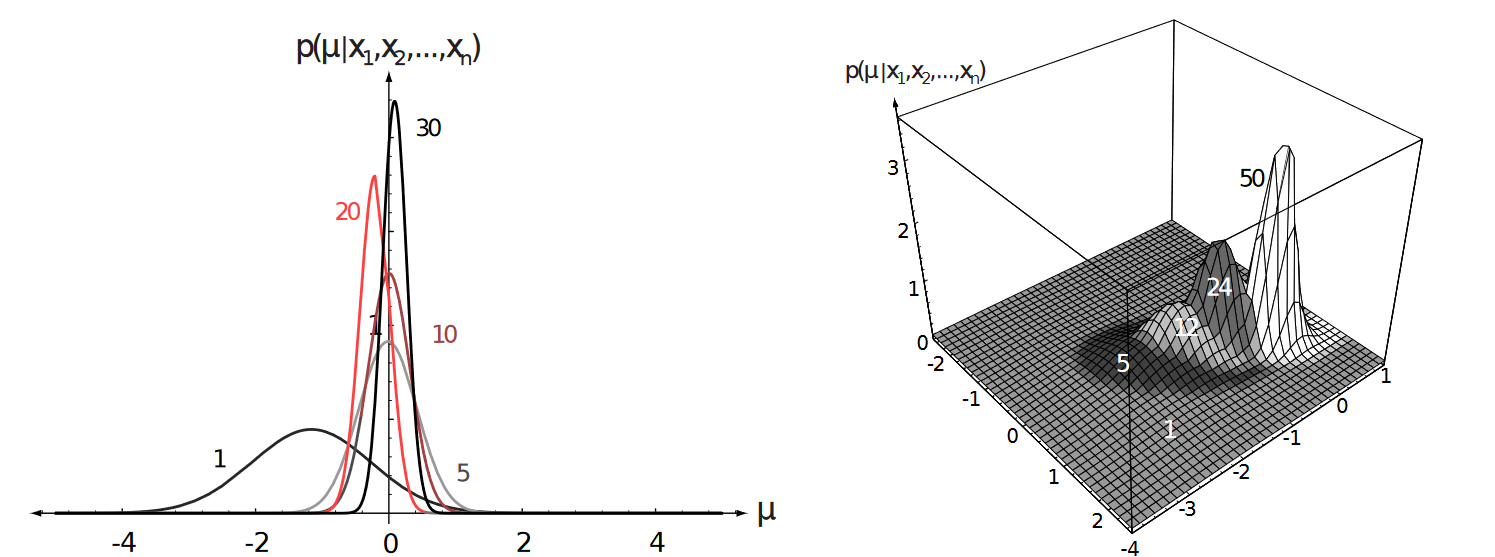
\includegraphics[scale=0.3]{
		images/07_ParameterEstimation_bayesianEstimation.png
	}
	\caption{2D and 3D graphics of increasing number of $n$ samples seen for a
	Bayesian estimation of the mean $\mu$}
	\label{fig:bayesian_mean_estimate}
\end{figure}

\sumup{ By this, we get that \[p(x|\mathcal{D}) \sim \mathcal{N}(\mu_{n}, \sigma^{2}+ \sigma_{n}^{2})\] therefore the Gaussian distribution of the probability for the new samples in the model is built with parameters $\Theta$ that are the mean (as the posterior mean) and the sum of the known variance and the variance of the mean as a random variable (aka the uncertainty over the mean. }

\subsection{Generalization of univariate case}
Since we know that $p(x|\mu) \sim \mathcal{N}(\mu, \Sigma)$\\ $p(\mu) \sim \mathcal{N}
(\mu_{n}, \Sigma_{n})$\\ therefore
$p(\mu|\mathcal{D}) \sim \mathcal{N}(\mu_{n}, \Sigma_{n})$\\ and $p(x|\mathcal{D}
) \sim \mathcal{N}(\mu_{n}, \Sigma + \Sigma_{n})$
\vspace{2cm}

\section{Sufficient statistics}
\defi{\textbf{Statistic}\label{def:statistic}\\ Any function on a set of samples $\mathcal{D}$ is a statistic, a sufficient statistic \[\textbf{s}= \Phi(\mathcal{D})\] if respects the following statement: \[P(\mathcal{D}|\textbf{s}, \Theta) = P(\mathcal{D}|\textbf{s})\] If $\Theta$ is a random variable, a sufficient statistic \textbf{s} contains all the relevant information about $\mathcal{D}$ in order to get the same and correct probability: \[p(\Theta|\mathcal{D}, \textbf{s}) = \frac{p(\mathcal{D}| \Theta, \textbf{s})p(\Theta|\textbf{s})}{p(\mathcal{D}|\textbf{s})}= p(\Theta|\textbf{s})\] }
A sufficient statistic for a Gaussian distribution are sample mean and covariance.

\section{Conjugate priors}
\defi{\textbf{Conjugate prior}\label{def:conj_prior}\\ Given the likelihood function $p(x|\Theta)$ and the prior distribution $p(\Theta)$, then \[p(\Theta)\] is a conjugate prior for $p(x|\Theta)$ if the posterior distribution $p(\Theta|x)$ is in the same family as the prior $p(\Theta)$ }

\begin{table}[H]
	\centering
	\begin{tabular}{|c|c|c|}
		\hline
		\textbf{likelihood} & \textbf{Parameters}              & \textbf{Conjugate prior} \\
		\hline
		Binomial            & p (\textit{probability})         & Beta                     \\
		\hline
		Multinomial         & p (\textit{probability vector})  & Dirichlet                \\
		\hline
		Normal              & $\mu$ (\textit{mean})            & Normal                   \\
		\hline
		Multivariate Normal & $\mu_{i}$ (\textit{mean vector}) & Normal                   \\
		\hline
	\end{tabular}
	\caption{examples of distributions and their conjugate priors}
	\label{table:conj_priors}
\end{table}

In Table \ref{table:conj_priors} we report some examples of distributions and
their conjugate priors.\\

\subsection{Example of a Bernoulli distribution}
Given a Bernoulli distribution \ref{defi:bernoullo_dist} with events $x=1$ for \textit{success}
and $x=0$ for \textit{failure}, parameters $\Theta$ for success and $1-\Theta$
for failure and probability mass distribution
\[
	P(x|\Theta) = \Theta^{x}(1-\Theta)^{1-x}
\]
then the conjugate prior is a Beta distribution \ref{def:beta_dist} that depends
on $\alpha_{h}, \alpha_{t}$
\begin{align*}
	P(\Theta|\psi) & = P(\Theta|\alpha_{h}, \alpha_{t})                                                                        \\
	               & = \frac{\Gamma(\alpha)}{\Gamma(\alpha_{h})\Gamma(\alpha_{t})}\Theta^{\alpha_h -1}(1-\Theta)^{\alpha_t -1}
\end{align*}

\subsubsection{Maximum likelihood estimation}
\label{par:maximum_likelyhood_estim} For example, we can prove that given a
dataset $\mathcal{D}= \{H, H, T, T, T, H, H\}$ of $N$ iterations (like head/tail
toss results), then the likelihood function becomes
\[
	p(\mathcal{D}|\Theta) = \Theta^{h}(1-\Theta)^{t}
\]
The maximum likelihood parameter (maximizing the probability means compute the
gradient and zeroing it), we are interested in the derivation with respect to
$\Theta$, then the estimation becomes
\begin{align*}
	\pdv{}{\Theta}\log p(\mathcal{D}| \Theta) \longrightarrow \pdv{}{\Theta}h\log \Theta + t \log(1-\Theta) & = 0             \\
	h\frac{1}{\Theta}- t\frac{1}{1-\Theta}                                                                  & = 0             \\
	h(1-\Theta)                                                                                             & = t\Theta       \\
	\Theta                                                                                                  & = \frac{h}{h+t}
\end{align*}
By this we mean that $t, h$ are a sufficient statistic \ref{def:statistic}. The
best maximum likelihood parameters is the number of successes in the data among
the total.

\subsubsection{Bayesian estimation}
If we try to estimate the parameters through a Bayesian estimation
\ref{par:Bayesian_estimation}, then the conjugate prior will still be a Beta distribution
\ref{def:beta_dist}.\\ The posterior is proportional to $P(\mathcal{D}|\Theta)P(\Theta
|\psi)$ which comes from the Bayes' theorem \ref{theo:bayes} where
$P(\mathcal{D})$ is omitted (therefore the $\propto$ property and not $=$), but it
is also proportional to $P(\mathcal{D}|\Theta)P(\Theta,\psi)$ which is the prior
Beta distribution
\begin{align*}
	P(\Theta|\mathcal{D}, \psi) & \propto P(\mathcal{D}|\Theta)P(\Theta|\psi)                                  \\
	                            & \propto \Theta^{h}(1-\Theta)^{t}\Theta^{\alpha_h -1}(1-\Theta)^{\alpha_t -1}
\end{align*}
This proportions gets together very easily collecting parameters until
\[
	P(\Theta|\mathcal{D},\psi) \propto \Theta^{h+\alpha_h -1}(1 - \Theta)^{t +
	\alpha_t -1}
\]
that is a Beta distribution $\sim Beta(\alpha_{h}',\alpha_{t}')$ where parameters
$\alpha_{h}'= h+\alpha_{h}$ and $\alpha_{t}' = t + \alpha_{t}$. The posterior of
my parameters is again a Beta with a new pair of parameters $\alpha_{h}'$ and
$\alpha_{t}'$ which are derived from the sum of the real counts ($h, t$) and the
\textit{imaginary} counts ($\alpha_{t}, \alpha_{h}$).\\

Then the prediction for a new event given the data is the expected value of the
posterior Beta:
\begin{align*}
	P(x|\mathcal{D}) & = \int_{\Theta}P(x,\Theta|\mathcal{D})d\Theta                     \\
	                 & = \int_{\Theta}P(\Theta|\mathcal{D}) P(\Theta|\mathcal{D})d\Theta
\end{align*}
Since we need to integrate on a binary output (success, fail), then let's focus of
the success event ($P(x=1) =\Theta$) keeping in mind that $\Theta$ is a Beta distribution
(therefore its expected value is
$E[\Theta] = \frac{\alpha_{h}'}{\alpha_{h}' + \alpha_{t}'}$):
\begin{align*}
	P(x = 1 | \mathcal{D}) & = \int_{\Theta}\Theta P(\Theta|\mathcal{D}, \psi) d\Theta \\
	                       & = E[\Theta]                                               \\
	                       & = \frac{h + \alpha_{h}}{h + t + \alpha_{h}+ \alpha_{t}}
\end{align*}
by this we get that:
\begin{itemize}
	\item with high $t, h$ (seen results) then the parameters $\alpha_{t}, \alpha_{h}$
		become irrelevant, so this estimation becomes closer to the maximum
		likelihood estimation,

	\item with small $t, h$ (seen results) that the prior estimate counts more.
\end{itemize}

\subsection{Example with a multinomial distribution}
Let's remind the reader the settings for a multinomial distribution: we have a set
with $r$ possible outcomes $x \in \{x^{1}, \dots, x^{r}\}$ and for each outcome a
(possibly different) probability (the probability over the dataset given the
parameters of the distribution).\\ The one-hot encoding is defined as $x(x) = [z_{1}
(x), \dots, z_{r}(x)]$ with $z_{k}(x) = 1$ if $x = x^{k}$, 0 otherwise.\\ The
probability mass function for this distribution is
\[
	P(x|\Theta) = \prod_{k=1}^{r}\Theta_{k}^{z_k(x)}
\]
while its conjugate prior is a Dirichlet distribution \ref{def:diri_dist}:
\begin{align*}
	P(\Theta|\psi) & = P(\Theta|\alpha_{1}, \dots, \alpha_{r})                                                          \\
	               & = \frac{\Gamma(\alpha)}{\prod_{k=1}^{r}\Gamma (\alpha_{k})}\prod_{k=1}^{r}\Theta_{k}^{\alpha_k -1}
\end{align*}

Starting from an example: we have a series of data representing the forecast of the
past $r$ days as $\mathcal{D}= \{R, C, C, S, S, S, R, C\}$ with R as rainy, C as
cloudy and S as sunny. Each of the outcome has its own probability $\Theta_{R}, \Theta
_{C}, \Theta_{S}$. Since we have the number of times that R, C and R were detected,
overall we have probabilities
$\Theta_{C}^{\#C}, \Theta_{R}^{\#R}, \Theta_{S}^{\#S}$ therefore
$\Theta_{C}^{3}, \Theta_{R}^{2}, \Theta_{S}^{3}$.

\subsubsection{Maximum likelihood estimation}
We now try to estimate parameters for the multinomial distribution with the
maximum likelihood method \ref{par:maximum_likelihood_estim}. We are trying to maximize
the probability $P(\mathcal{D}|\Theta)$, therefore we look for the maximum of
the logarithmic function that describes the probability.
\[
	\nabla_{\Theta}\log P(\mathcal{D}|\Theta) = 0
\]
taking into account also that the sum of the probabilities need to be equal to 1
\[
	\sum_{i=1}^{n}\Theta_{i}= 1
\]
From these assumptions we get:
\[
	\Theta_{i}= \frac{N_{i}}{\sum_{i=1}^{n}N_{i}}
\]
which stands for the fraction of the outcomes in $\mathcal{D}$. Also, the
numbers of the different outcomes in $\mathcal{D}$ are a sufficient statistic
\ref{def:statistic}.

\subsubsection{Bayesian estimation}
Let's now try to estimate the parameters with the Bayesian method
\ref{par:Bayesian_estimation}. In this case we have to consider that
\begin{align*}
	P(\Theta|\mathcal{D}) & \propto P(\mathcal{D}|\Theta)P(\Theta)                                         \\
	                      & \propto \prod_{i=1}^{r}\Theta_{i}^{N_i}\prod_{i=1}^{r}\Theta_{i}^{\alpha_i -1}
\end{align*}
where $P(\Theta|\mathcal{D})$ is the posterior, $P(\Theta)$ is the prior (Dirichlet
distribution \ref{def:diri_dist}) and $P(\mathcal{D}|\Theta)$ is the likelihood.\\
Then we have that
\begin{align*}
	\prod_{i=1}^{r}\Theta_{i}^{N_i}\prod_{i=1}^{r}\Theta_{i}^{\alpha_i -1} & = \prod_{i=1}^{r}\Theta^{N_i + \alpha_i -1} \\
	                                                                       & = \prod_{i=1}^{r}\Theta^{\alpha' -1}
\end{align*}
Fixing $\alpha' = N_{i}+ \alpha_{i}$.\\

Let's take for example the computation for $x=R$, then
\begin{align*}
	P(x=R|\mathcal{D}) & = \int_{\Theta}P(x=R|\Theta)P(\Theta|\mathcal{D}) d\Theta \\
	                   & = \int_{\Theta}\Theta_{R}P(\Theta_{R}|\mathcal{D})d\Theta \\
	                   & = E[\Theta_{R}]
\end{align*}
we end up with the expected value for \textit{R}.
\begin{align*}
	E[\Theta_{R}] & = \frac{\alpha_{R}'}{\sum_{i=1}^{r}\alpha_{i}'}             \\
	              & = \frac{N_{r}+ \alpha_{R}}{\sum_{i=1}^{r}N_{i}+ \alpha_{i}}
\end{align*}

Also in this case, the prediction ends up being influenced by the actual seen
values in $N_{R}$ but also partially driven by the \textit{imaginary} value for the
parameter estimation $\alpha_{R}$.
